\section{Durchführung}

\subsection{Aufnahme der Kennlinien}
Die zur Messung der Kennlinien benötigte Schaltung ist in Abbildung \ref{fig:schaltung_kennlinie} zu sehen.
Dabei wird der XY-Schreiber allerdings nicht verwendet.
Mit Hilfe eines regelbaren Konstantspannungsgeräts wird eine Heizspannung $U_\text{f}$ und ein Heizstrom $I_\text{f}$ erzeugt,
die am Gerät selbst abgelesen werden können.
Die verwendete Diode darf maximal mit $I_\text{f} = \qty[]{2.5}{\ampere}$ betrieben werden.
Die Anodenspannung $U_\text{A}$ kann mit einem weiteren regelbaren Gleichspannungsgerät betrieben werden, welches die Messwerte für 
$U_\text{A}$ und $I_\text{A}$ anzeigt.
Dabei ist $I_\text{A}$ auf $\qty[]{2}{\milli\ampere}$ beschränkt.

\begin{figure}
    \centering
    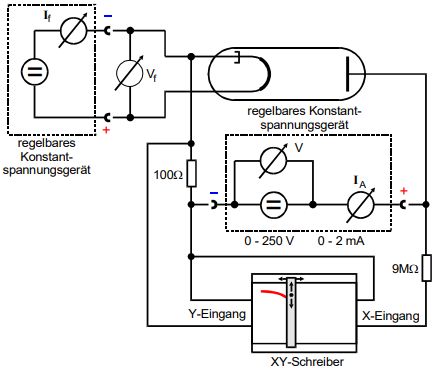
\includegraphics[height = 7cm]{Abbildungen/schaltung_kennlinie.png}
    \caption{Schaltplan zur Aufnahme der Kennlinien \cite[]{man:v504}.}
    \label{fig:schaltung_kennlinie}
\end{figure}

\noindent
Zum Aufzeichnen einer Kennlinienschar werden insgesamt drei Messreihen mit verschiedenen $I_\text{f}$ durchgeführt.
Bei der ersten Reihe beträgt $I_\text{f} = \qty[]{2.0}{\ampere}$, danach $\qty[]{2.3}{\ampere}$ und schließlich $\qty[]{2.5}{\ampere}$.
Die entsprechenden Heizspannungen betragen dabei $U_\text{f} = \qty[]{4}{\volt}$ und danach je $\qty[]{5}{\volt}$.
In jeder Messreihe wird die Anodenspannung $U_\text{A}$ so weit erhöht bis entweder ein Sättigungsstrom eingetreten ist oder
eine Maximalspannung von $\qty[]{250}{\volt}$ erreicht wurde.



\subsection{Messung der Anlaufstromkurve}
Der Schaltplan zur Messung des Anlaufstroms ist in Abbildung \ref{fig:schaltung_anlaufstrom} zu sehen.
Anstatt den Anodenstrom direkt über das Spannungsgerät zu messen wird ein empfindlicheres Nanoamperemeter verwendet, 
um die geringeren Werte im $\unit{\nano\ampere}$-Bereich messen zu können.
Aufgrund der geringen Größenordnung sollte die Leitung zwischen Anode und Nanoamperemeter so kurz wie möglich sein.
Weiterhin ist zu beachten, dass das Nanoamperemeter einen Innenwiderstand von $R_\text{i} = \qty[]{1}{\mega\ohm}$ hat, 
weshalb die angezeigte Spannung $U_\text{A}$ nicht dem tatsächlichen Wert entspricht.

\begin{figure}
    \centering
    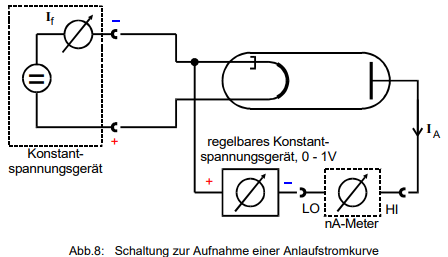
\includegraphics[height = 5cm]{Abbildungen/schaltung_anlaufstrom.png}
    \caption{Schaltplan zur Messung des Anlaufstroms \cite[]{man:v504}.}
    \label{fig:schaltung_anlaufstrom}
\end{figure}

\noindent
Zum Messen des Anlaufstroms wird bei der maximalen Heizspannung von $\qty[]{2.5}{\volt}$ die angezeigte Anodenspannung $U_\text{A}$
ausgehend von $\qty{0}{\volt}$ so weit verringert, bis kein Strom mehr messbar ist.
Dabei muss gelegentlich die Empfindlichkeit des Nanoamperemeters angepasst werden.
Die entsprechenden Strom- und Spannungswerte werden notiert.
